\documentclass{beamer}
\usepackage{beamerthemesplit}
\usepackage{wrapfig}
\usetheme{SPbGU}
\usepackage{pdfpages}
\usepackage{amsmath}
\usepackage{cmap} 
\usepackage[T2A]{fontenc} 
\usepackage[utf8]{inputenc}
\usepackage[english,russian]{babel}
\usepackage{indentfirst}
\usepackage{amsmath}
\usepackage{tikz}
\usepackage{dot2texi}
\usepackage{multirow}
\usepackage{fancyvrb}
\usepackage{graphicx}
\usepackage{array}
\usepackage{subcaption}
\usepackage[noend]{algpseudocode}
\usepackage{algorithm}
\usepackage{algorithmicx}
\usetikzlibrary{shapes,arrows}
\usepackage{fancyvrb}
\usepackage[normalem]{ulem} % для подчёркиваний uline
\newtheorem{rutheorem}{Теорема}
\newtheorem{ruproof}{Доказательство}
\newtheorem{rudefinition}{Определение}
\newtheorem{rulemma}{Лемма}
\beamertemplatenavigationsymbolsempty


\title[]{Обзор задач синтаксического анализа графов}
\subtitle[]{В рамках проекта лаборатории JetBrains}
% То, что в квадратных скобках, отображается в левом нижнем углу. 
\institute[СПбГУ]{
Санкт-Петербургский государственный университет \\
Кафедра системного программирования }

% То, что в квадратных скобках, отображается в левом нижнем углу.
\author[Рустам Азимов]{Рустам Шухратуллович Азимов, 546 группа \\
  % У научного руководителя должна быть указана научная степень
  \and  
    {\bfseries Научный руководитель:} к.ф.-м.н., ст.пр. С.В. Григорьев}

\date{27 декабря 2016г.}

\definecolor{orange}{RGB}{179,36,31}

\begin{document}
{
% Лого университета или организации, отображается в шапке титульного листа
\begin{frame}
  \begin{center}
  {
\includegraphics[width=1cm]{pictures/SPbGU_Logo.png}}
  \end{center}
  \titlepage
\end{frame}
}

\begin{frame}[fragile]
  \transwipe[direction=90]
  \frametitle{Синтаксический анализ графов}
  \begin{itemize}
    \item Граф --- коллекция генеалогических деревьев
    \item Вершины графа --- люди
    \item Ребра представляют отношение между родителями и детьми ($parentOf$ или $childOf$)
    \item Формальный КС-язык $L$ = \{$parentOf$^{n}$childOf^{n} | n > 0\}$
    \item Пути, соответствующие языку $L$, соединяют потомков общего предка из одного поколения
  \end{itemize}
\end{frame}

\begin{frame}[fragile]
	\transwipe[direction=90]
	\frametitle{Проблемы}
	\begin{itemize}
	    \item Существует множество вариаций задач синтаксического анализа графов
	    \item Работы в данной области по-разному формулируют задачи и используют различную терминологию
	    \item Сложность использования существующих результатов данной области (например, обобщение этих результатов с использованием других классов формальных языков)
    \end{itemize}
\end{frame}

            
\begin{frame}[fragile]
	\transwipe[direction=90]
	\frametitle{Постановка задачи}
	 \textbf{Цель:} обзор существующих результатов для различных задач синтаксического анализа графов
    \begin{itemize}
        \item Изучить литературу, посвящённую решению задач синтаксического анализа графов
        \item Выявить основные классы задач синтаксического анализа графов и их ключевые характеристики
        \item Составить общую таблицу, отражающую связь классов задач и характеристик
    \end{itemize}
\end{frame}

\begin{frame}[fragile]
	\transwipe[direction=90]
	\frametitle{Работы в области синтаксического анализа графов}
    \begin{itemize}
        \item Barrett C., Jacob R., Marathe M. Formal language constrained path problems
        \item Hellings J. Conjunctive context-free path queries
        \item Sevon P., Eronen L. Subgraph queries by context-free grammars
        \item Hellings J. Path results for context-free grammar queries on graphs
        \item Yannahzkis M. Graph-theoretic methods in database theory
    \end{itemize}   
\end{frame}

\begin{frame}[fragile]
	\transwipe[direction=90]
	\frametitle{Классы задач синтаксического анализа графов}
    \begin{itemize}
        \item \textbf{Семантика запроса}
            \begin{itemize}
                \item кратчайший путь из вершины $s$ в вершину $d$
                \item простой путь из вершины $s$ в вершину $d$
                \item выделение подграфа связей
            \end{itemize}
        \item \textbf{Тип графа}
            \begin{itemize}
                \item без циклов
                \item планарный
                \item без ограничений
            \end{itemize}
        \item \textbf{Класс формального языка}
            \begin{itemize}
                \item регулярный
                \item контекстно-свободный
                \item конъюнктивный
            \end{itemize}
    \end{itemize}   
\end{frame}

\begin{frame}[fragile]
	\transwipe[direction=90]
	\frametitle{Общая таблица}
	\begin{center}
	            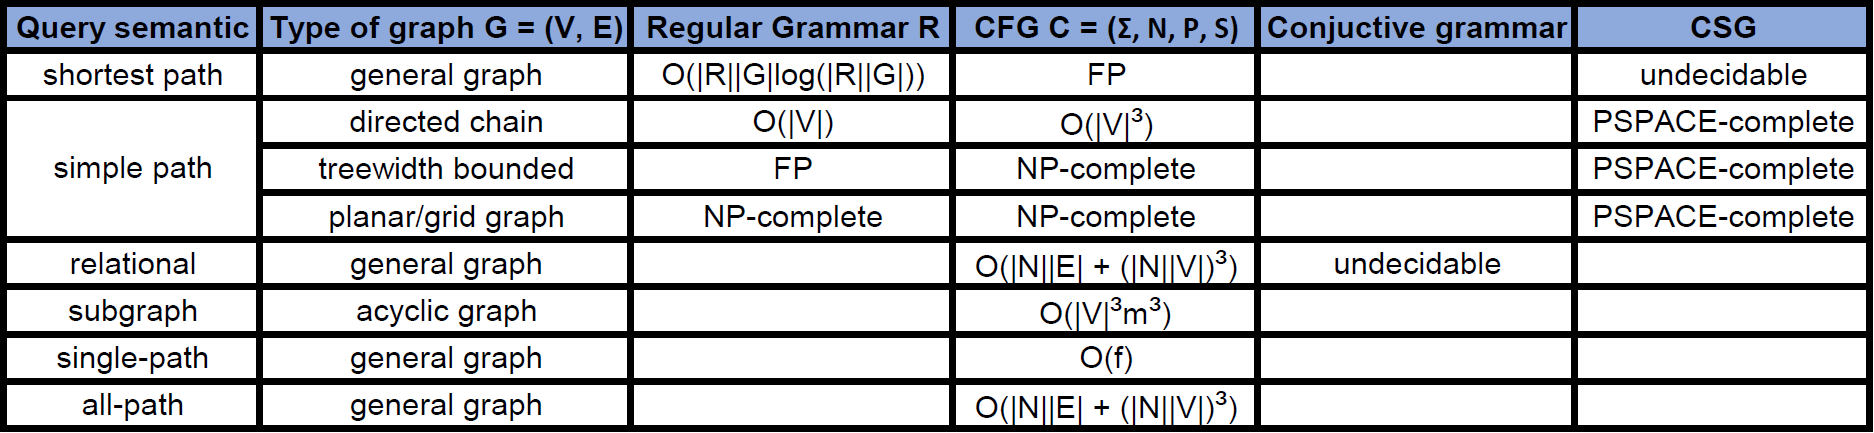
\includegraphics[width=340pt]{pictures/table_short.png}
	\end{center}
	Здесь $m$ означает максимальную длину пути в графе, а $f = |N||V|^{2}((|N||V|^{2}) log(|N||V|^{2}) + |P||V|^{3} + min(|N|,|P|) |E|) + 2^{|N||V|^{2} - 1}$
\end{frame}

\end{document}